\subsection{Web application}
	La componente \textit{web app} ha il compito di interfacciare gli utenti con i dispositivi censiti dal sistema e visibili al loro ente di appartenenza.
	\newline
	Le principali funzionalità messe a disposizione riguardano la visualizzazione di grafici contenenti i dati di determinati sensori, la modifica delle configurazioni dei gateway e l'aggiunta o la rimozione di dispositivi e/o sensori.
	\newline 
	La componente è stata sviluppata utilizzando i framework Laravel e Vue.js.
	
	\subsubsection{Diagramma dei package}%%%%%%%%%OK
		\begin{figure}[H]
			\centering
			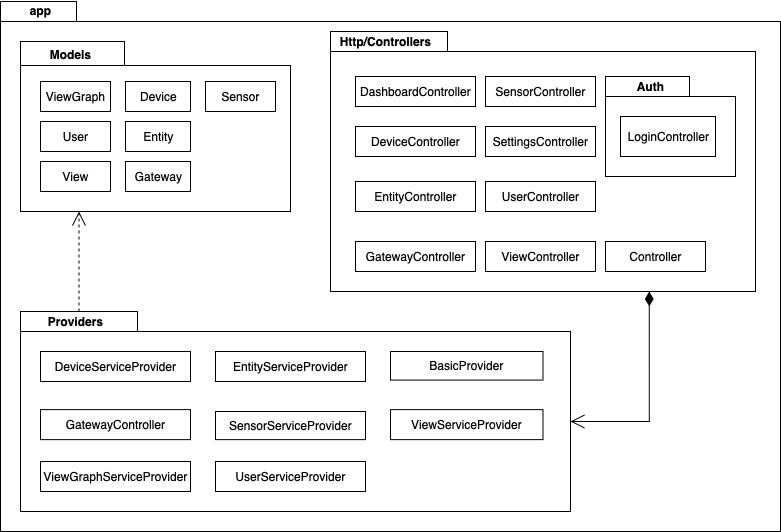
\includegraphics[scale=0.450]{res/images/WEBAPP/WebAppPackage.png}
			\caption{Diagramma dei package della componente web app}
			\label{Diagramma 21}
		\end{figure}
	
	\subsubsection{Dipendenze esterne}
		La componente ha le seguenti dipendenze esterne:
		\begin{itemize}
			\item \textbf{Laravel:} framework alla base della web app, da cui vengono prese le basi dei controllers e dei models. Inoltre è il gestore delle view;
			\item \textbf{Laravel/UI:} viene utilizzata per l'autenticazione all'interno della web app;
			\item \textbf{guzzlehttp/guzzle:} viene utilizzata per effettuare richieste HTTP in linguaggio PHP;
			\item \textbf{Axios:} viene utilizzata per effettuare delle richieste HTTP in JavaScript;
			\item \textbf{Datatables.js:} viene utilizzata per la paginazione delle tabelle;
			\item \textbf{Apexcharts:} viene utilizzata per fare i grafici visibili all'interno dell'applicazione web;
			\item \textbf{davejamesmiller/laravel-breadcrumbs:} questa dipendenza viene utilizzata per generare i breadcrumb all'interno delle pagine visualizzate;
			\item \textbf{Vue.js:} framework che permette, tra le altre cose, di utilizzare array e variabili all'interno delle pagine per permetterne una visualizzazione dinamica dei contenuti;
			\item \textbf{Bootstrap:} framework utilizzato per la creazione dell'interfaccia grafica dell'applicazione web;
			\item \textbf{JQuery:} libreria utilizzata da Bootstrap per molte delle sue componenti;
			\item \textbf{Popper.js:} altra libreria utilizzata da Bootstrap.
		\end{itemize}



	\subsubsection{Diagrammi delle classi}%%%%%%%%%%OK
	Nel diagramma delle classi della componente web app, rappresentato nel file \textit{Immagini/WebApp-Classi.png}, sono presenti principalmente i provider ed i controller: i provider sono le componenti che effettuano le richieste API da parte della web app e lavorano quindi a basso livello.
	\newline
	I controller invece dialogano con i provider ad un livello di astrazione più alto. Le pagine view non sono presenti in quanto il framework Laravel le gestisce tramite pagine HTML.
	\begin{landscape}
	\subsubsection{Diagrammi di sequenza}%%%%%%%%%%OK
		\begin{figure}[H]
			\centering
			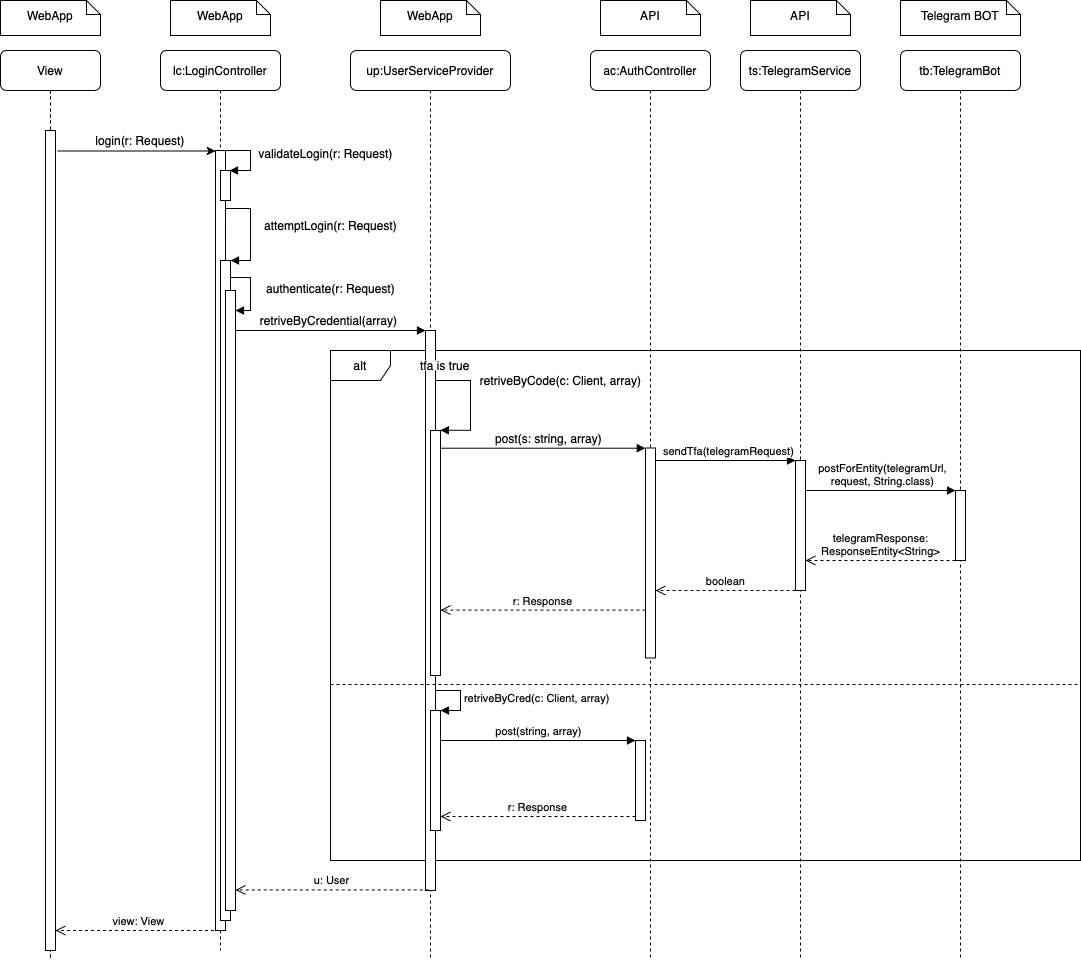
\includegraphics[scale=0.400]{res/images/WEBAPP/AutenticazioneTfa.png}
			\caption{Diagramma di sequenza che illustra l'autenticazione all'interno della componente web app}
			\label{Diagramma 23}
		\end{figure}
		Nel diagramma di sequenza che rappresenta l'autenticazione, alla richiesta della vista di effettuare l'autenticazione, il LoginController verifica che le credenziali siano corrette ed in seguito, se l'utente ha attivato l'autenticazione a due fattori, invia il codice tramite richiesta HTTP POST al bot di Telegram, il quale visualizza il codice nella chat dell'utente.
		\newline
		Mentre, se l'utente non l'ha attivata, invia semplicemente la risposta all'utente. In entrambi i casi viene mostrata la risposta affermativa o negativa all'utente e se positiva viene effettuata l'autenticazione.
		\begin{figure}[H]
			\centering
			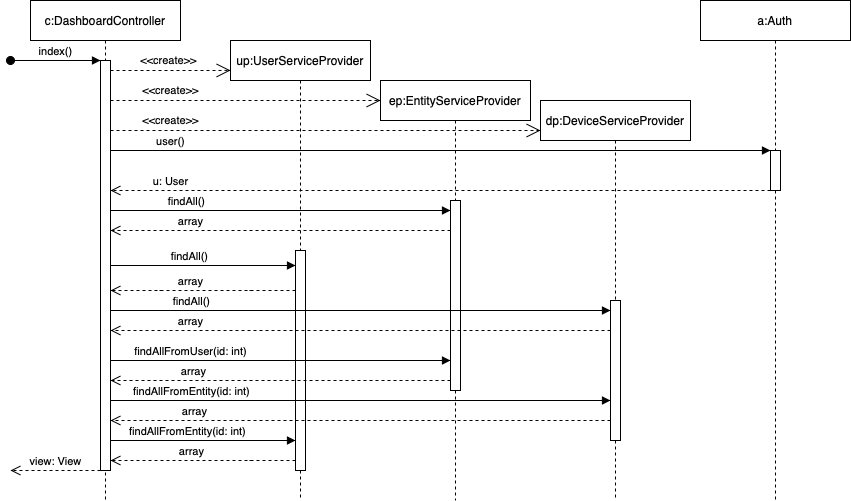
\includegraphics[scale=0.600]{res/images/WEBAPP/Dashboard.index.png}
			\caption{Diagramma di sequenza che illustra la visualizzazione della schermata dashboard all'interno della componente web app}
			\label{Diagramma 24}
		\end{figure}
		Come si evince dal diagramma, il DashboardController crea uno UserService, un EntityServiceProvider ed un DeviceServiceProvider, i quali effettuano le richieste API per richiedere le informazioni da visualizzare nella dashboard, quali ad esempio il numero di utenti di un certo ente o le informazioni dell'account dell'utente che sta visualizzando la dashboard. Infine tutte le informazioni ricavate vengono restituite alla pagine view.
	\end{landscape}